% !TEX root = ../thesis-example.tex
%
\chapter{Algorytmy korejestracji przestrzennej obrazów OCT}
\label{sec:algorytmy_korejestracji}

\textbf{Mozaiką} nazywa się obraz powstały poprzez połączenie grupy obrazów zwanych w żargonie ,,kafelkami'' na podstawie ich wzajemnych relacji. Znanym oraz popularnym przykładem łączenia obrazów w jeden większy jest funkcja panoramy w telefonach komórkowych czy aparatach fotograficznych. Od strony użytkownika proces tworzenia panoramy polega na powolnym przesuwaniu telefonem po linii poziomej do momentu aż żądany krajobraz zostanie uchwycony. Od strony urządzenia proces polega na wykonywaniu serii zdjęć oraz następnie łączenie nachodzących klatek w jeden obraz. Rezultatem jest jednolita panorama, która składa się z grupy mniejszych węższych zdjęć.

Celem niniejszej pracy jest stworzenie mozaiki OCT (przykład na rysunku \ref{fig:algorytmy_korejestracji:mosaic}) z połączenia mniejszych nachodzących na siebie nawzajem angiograficznych obrazów OCT (przykład obrazu angiograficznego OCT znajduje się z prawej strony na rysunku \ref{fig:obrazowanie_oct:bscan_vessels}).

\begin{figure}[H]
  \centering
  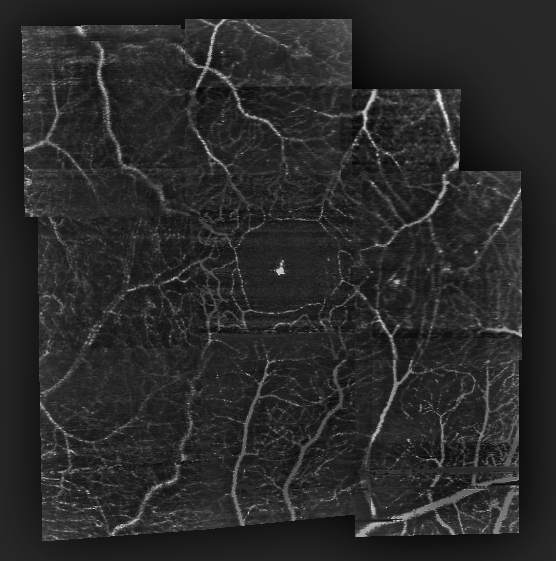
\includegraphics[width=10cm]{gfx/mosaic}
  \caption{Mozaika OCT stworzona z połączenia angiograficznych obrazów OCT.}
  \label{fig:algorytmy_korejestracji:mosaic}
\end{figure}

Proces automatycznego stworzenia mozaiki (ang. \textit{stitching}) takiej jak na rysunku \ref{fig:algorytmy_korejestracji:mosaic} jest zadaniem nietrywialnym i wymaga dokładnej analizy wiedzy dziedzinowej oraz precyzyjnego wyboru metod przetwarzania obrazów. Pierwszym krokiem jest wybór modelu deformacji kafelków (sekcja \ref{sec:algorytmy_korejestracji:model_deformacji}), następnym etapem jest wybór metody wzajemnej korejestracji kafelków (sekcja \ref{sec:algorytmy_korejestracji:korejestracja_kafelow}). Posiadając zdefiniowane wzajemne relacje kafelków oraz ich docelowe położenie w finalnej mozaice należy wykonać proces łączenia kafelków (sekcja \ref{sec:algorytmy_korejestracji:laczenie_kafelkow}). W każdej z tych sekcji jest wyjaśniona idea metody w kontekście stworzenia mozaiki OCT, natomiast szczegółowy opis zaimplementowanych metod znajduje się w rozdziale \ref{sec:proponowane_algorytmy}.

\section{Model deformacji kafelków}
\label{sec:algorytmy_korejestracji:model_deformacji}

Model deformacji kafelków określa dozwolone przekształcenia geometryczne odwzorowujące piksele kafelka do pikseli kafelka w finalnej mozaice. Ze względu na to, że angiograficzne obrazy OCT znajdują się na jednej płaszczyźnie\footnote{W rzeczywistości powierzchnia siatkówki jest wklęsła. Uproszenie polegające na przedstawieniu mozaiki na płaszczyźnie znacznie ułatwia implementację, a nie powoduje widocznych zniekształceń.} możliwy zbiór modeli deformacji ogranicza  się do transformacji dwuwymiarowych przedstawionych na rysunku \ref{fig:algorytmy_korejestracji:trans}.

\begin{figure}[H]
  \centering
  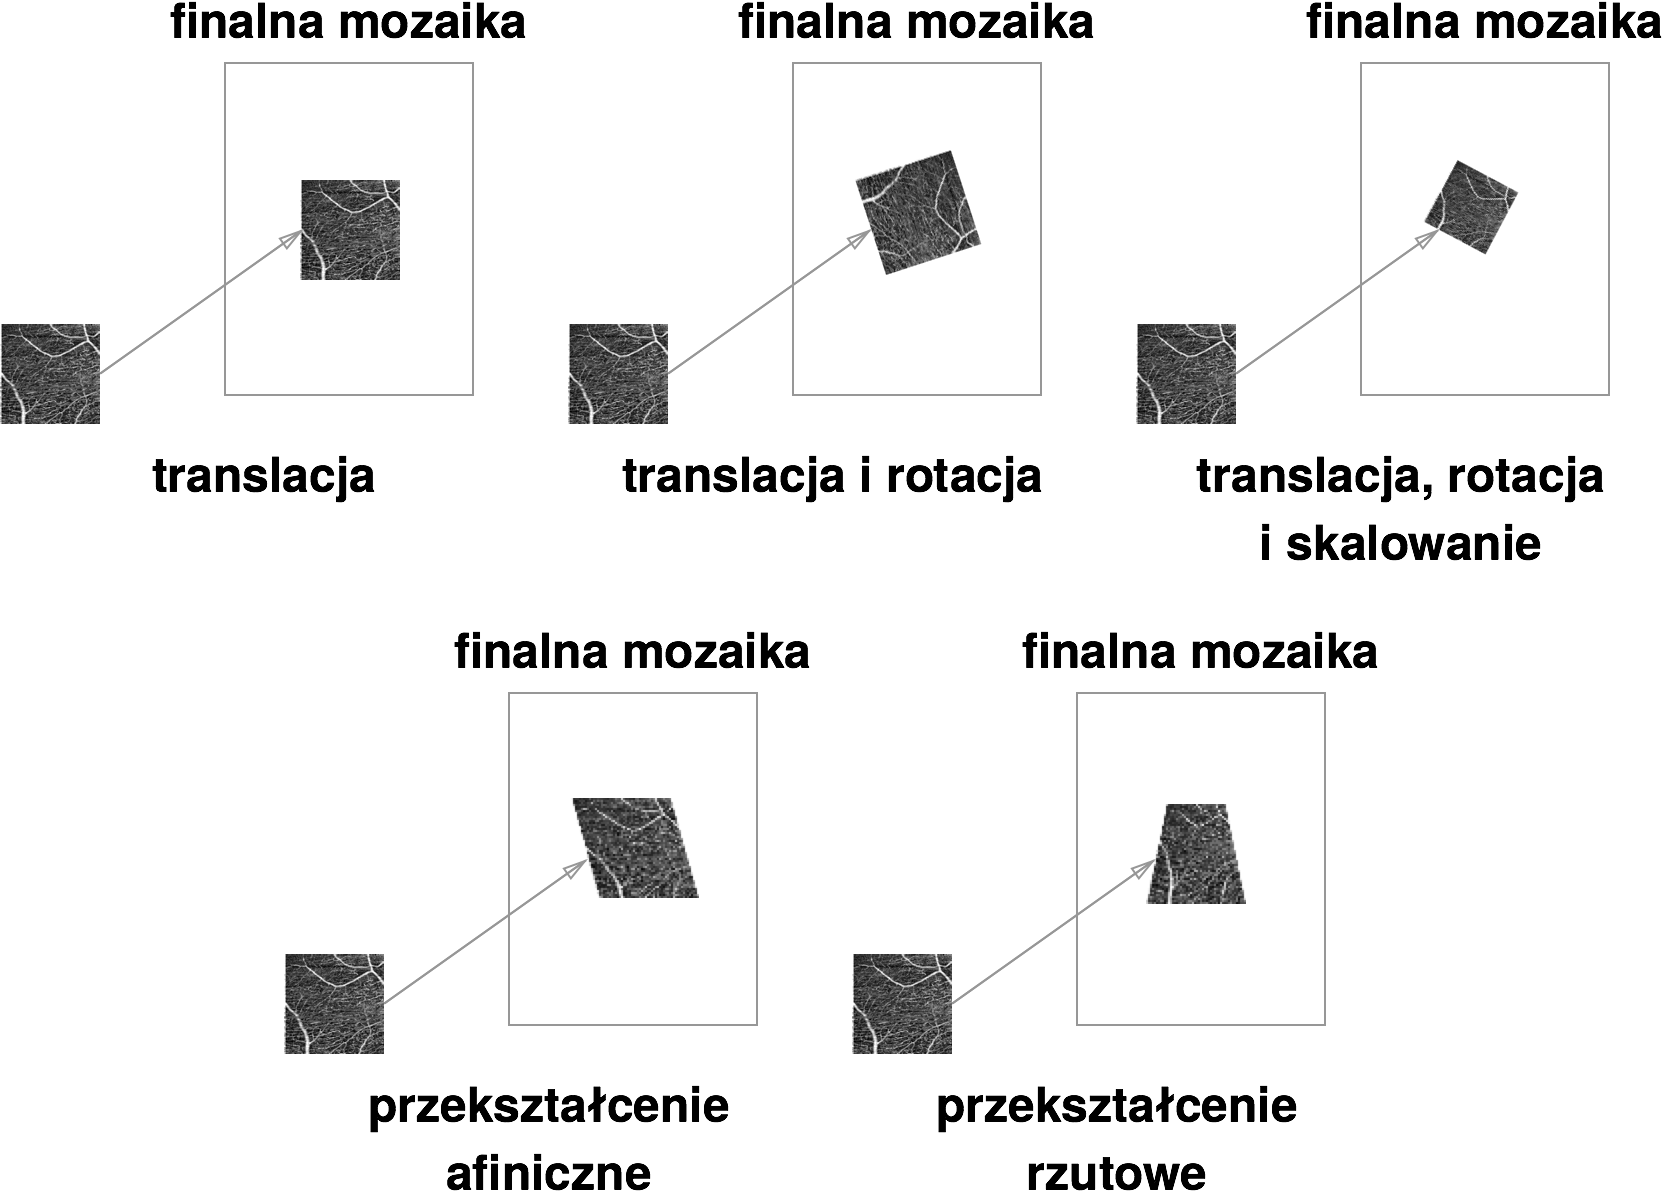
\includegraphics[width=\textwidth]{gfx/trans}
  \caption{Zbiór transformacji dwuwymiarowych dla przykładowego angiograficznego obrazu OCT.}
  \label{fig:algorytmy_korejestracji:trans}
\end{figure}

Idealnie OCT powinno tworzyć obrazy angiograficzne, które są względem siebie tylko przesunięte. W rzeczywistości pojawiają się zniekształcenia wynikające z niedokładności urządzenia oraz ruchu oka pacjenta, przez co niektóre kafelki są nieznacznie obrócone względem siebie. Z tego względu wybranym modelem deformacji kafelków został \textbf{model transformacji ciała sztywnego}, czyli połączenie translacji i rotacji.

\subsection{Matematyczny zapis modelu transformacji ciała sztywnego}

Współrzędne piksela w kafelku to trójelementowy wektor $\widetilde{x}=(x, y, 1)$, gdzie $x$ i $y$ to współrzędne piksela w układzie współrzędnych kafelka. Tak zdefiniowany piksel poddaje się transformacji ciała sztywnego. Po transformacji piksel posiada współrzędne $\hat{x}=(x', y')$ w układzie współrzędnych finalnej mozaiki. Transformacja ciała sztywnego jest zdefiniowana następująco:
\begin{equation}
\hat{x}=\begin{bmatrix}R&t\end{bmatrix}\widetilde{x}
\label{eq:transformation}
\end{equation}
gdzie:

\begin{align}
R &= \begin{bmatrix}cos(\theta)&-sin(\theta)\\sin(\theta)&cos(\theta)\end{bmatrix} &&\text{i} & t &= \begin{bmatrix}t_{x}\\t_{y}\end{bmatrix}
\label{eq:rotation_and_translation}
\end{align}

W równaniu \ref{eq:rotation_and_translation} $\theta$ to kąt obrotu (rotacja) względem początku układu współrzędnych, a $t_{x}$ i $t_{y}$ to odpowiednio przesunięcia względem osi x i osi y. Parametry $\theta$, $t_{x}$ i $t_{y}$ są niewiadomymi równania \ref{eq:transformation}, których obliczenie jest wyjaśnione w sekcji \ref{sec:algorytmy_korejestracji:korejestracja_kafelow}.

\section{Korejestracja kafelków}
\label{sec:algorytmy_korejestracji:korejestracja_kafelow}

Po wyborze modelu deformacji kafelków można przejść do wyboru metody określającej jego parametry (w przypadku niniejszej pracy są to parametry przesunięcia i obrotu). Metoda powinna zwrócić takie wartości by kafelek znalazł się w odpowiednim miejscu w finalnej mozaice z możliwie najmniejszym błędem. By rozwiązać ten problem najpierw trzeba poznać położenie kafelków względem siebie oraz ustalić kafelek referencyjny. Rysunek \ref{fig:algorytmy_korejestracji:reference_tile} przedstawia przykładowe rozmieszczenie kafelków. Kafelek referencyjny oznaczony przerywaną linią jest jedynie poddany translacji, natomiast żeby odpowiednio umieścić kafelki (2) i (3) trzeba najpierw znać dopasowanie kafelków (2) i (3) do kafelka referencyjnego (1). W przykładzie na rysunku \ref{fig:algorytmy_korejestracji:reference_tile} zostało założone, że kafelki (2) i (3) mogą być dopasowane do kafelka (1). Informacja na temat relacji geometrycznych pomiędzy kafelkami wynika z wiedzy dziedzinowej (sekcja \ref{sec:proponowane_algorytmy:wiedza_dziedzinowa}).

\begin{figure}[H]
  \centering
  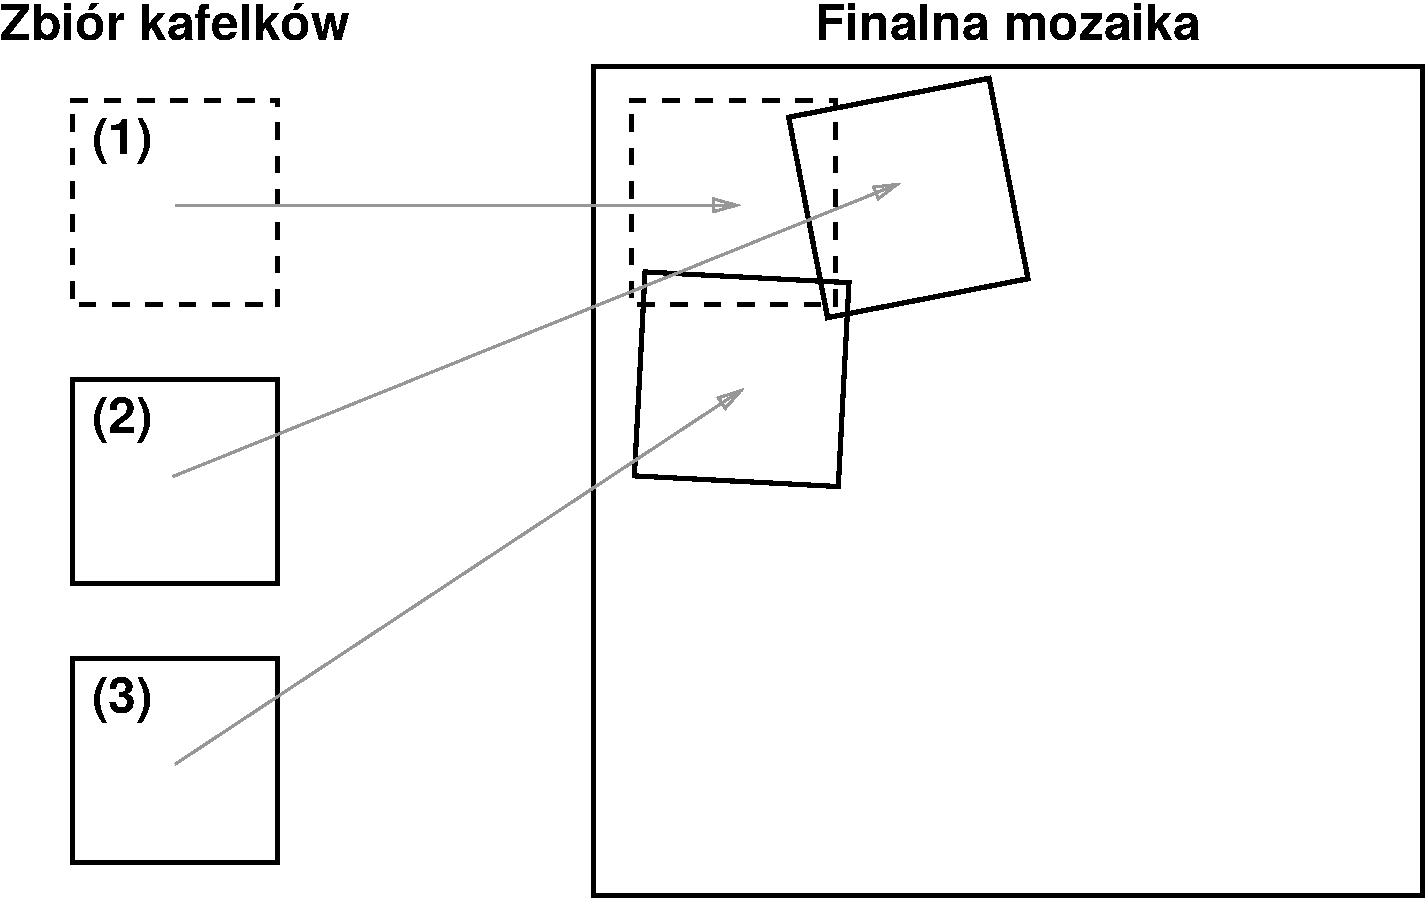
\includegraphics[width=\textwidth]{gfx/reference_tile}
  \caption{Przykładowe rozmieszczenie kafelków na finalnej mozaice. Kafelek referencyjny jest wyróżniony przerywaną linią.}
  \label{fig:algorytmy_korejestracji:reference_tile}
\end{figure}

Dopasowanie dwóch kafelków do siebie nazywa się również ich korejestracją, czyli przeniesieniem dwóch kafelków do wspólnego układu współrzędnych w taki sposób by były względem siebie dopasowane. Prosty przykład korejestracji przedstawiony jest na rysunku \ref{fig:algorytmy_korejestracji:align}, gdzie kafelki mają wspólny obszar nałożenia.

\begin{figure}[H]
  \centering
  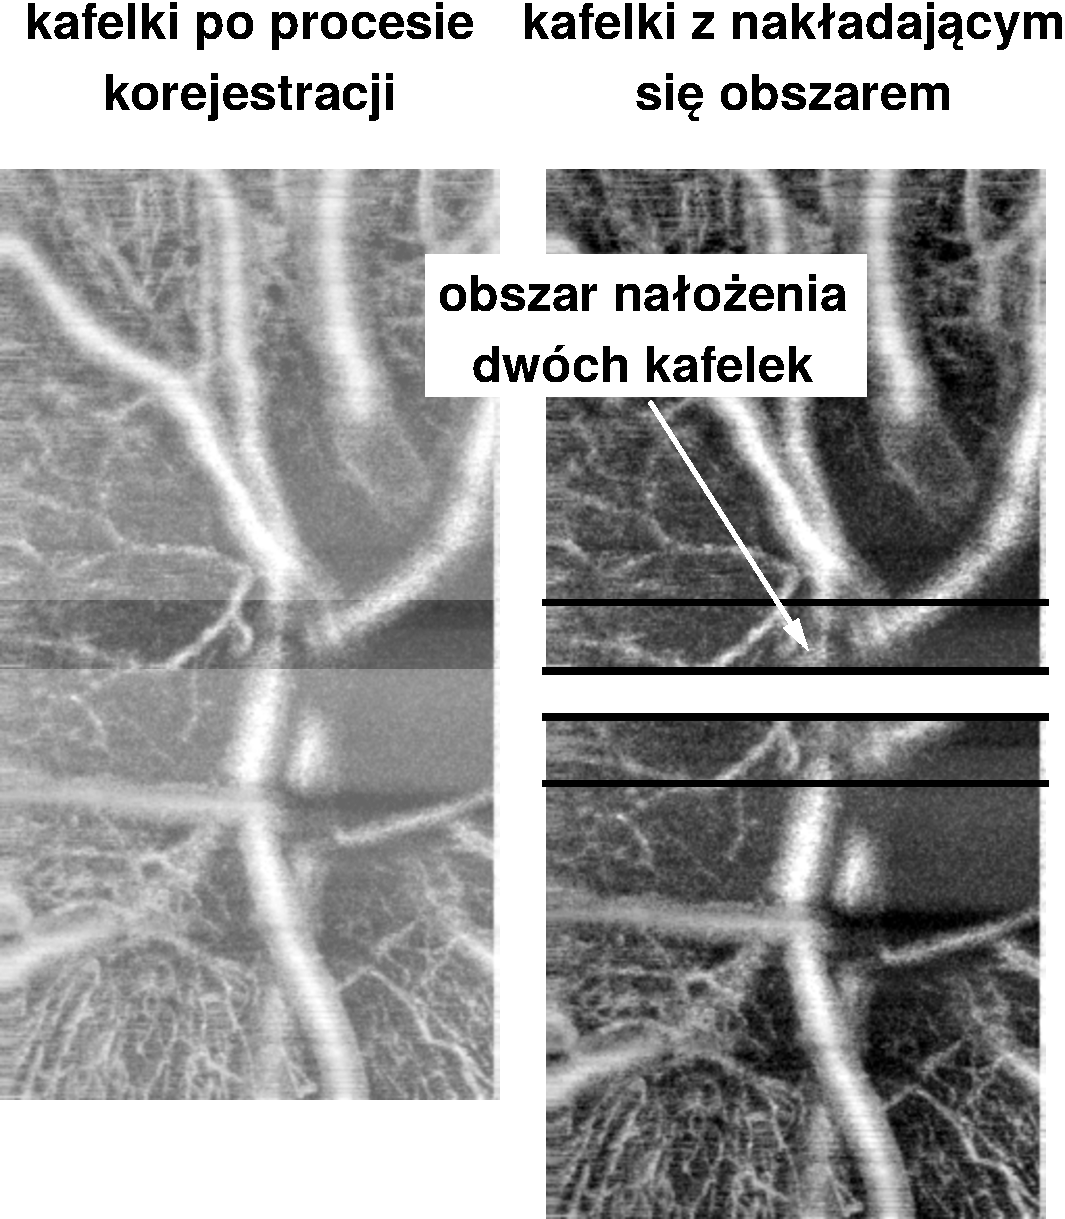
\includegraphics[width=7cm]{gfx/align}
  \caption{Przykładowa korejestracja dwóch kafelków ze wspólnym obszarem nałożenia.}
  \label{fig:algorytmy_korejestracji:align}
\end{figure}

Dopasowanie kafelków z rysunku \ref{fig:algorytmy_korejestracji:align} jest przykładem bardzo prostym, ponieważ wymaga tylko translacji jednego kafelka względem drugiego. W rzeczywistości pomiary OCT nie są tak dokładne. Prosta translacja wzdłuż jednej z osi nie wystarcza, przez co wymagane jest użycie metody automatycznie wyznaczającej parametry translacji i rotacji. Dwie najpopularniejsze metody to:

\begin{enumerate}
\item \textbf{Korejestracja na podstawie wartości pikseli} (sekcja \ref{sec:algorytmy_korejestracji:korejestracja_na_podstawie_wartosci}) - Metoda wielokrotnie przesuwająca jeden obraz względem drugiego i następnie oceniająca każdą z tych unikalnych pozycji pod względem dopasowania obrazów do siebie.
\item \textbf{Korejestracja na podstawie cech} (sekcja \ref{sec:algorytmy_korejestracji:korejestracja_na_podstawie_cech}) - Metoda ekstrahująca charakterystyczne cechy z każdego obrazu i następnie dopasowująca te cechy by osiągnąć globalną spójność. Dopasowania są później użyte przez algorytm do wyznaczenia macierzy transformacji pomiędzy obrazami.
\end{enumerate}

\subsection{Korejestracja na podstawie wartości pikseli}
\label{sec:algorytmy_korejestracji:korejestracja_na_podstawie_wartosci}

Korejestracja na podstawie wartości pikseli jest często nazywana metodą bezpośrednią, ponieważ wymaga bezpośredniego porównania wartości pikseli nakładających się obrazów. Pierwszym krokiem w tej metodzie jest wybranie odpowiedniej miary błędu. Taką miarą błędu może być funkcja suma błędów kwadratowych $E_{RSS}$ (ang. \textit{residual sum of squares, RSS}). Mając daną funkcję $I_{S}(p_{i})$ zwracającą wartość piksela w obrazie źródłowym (przesuwanym) w lokalizacji $p_{i}=(x_{i}, y_{i})$ oraz funkcję $I_{T}(p_{i})$ zwracającą wartość piksela w obrazie docelowym (referencyjnym, pozostającym na miejscu) $E_{RSS}$ można zdefiniować jako:
\begin{equation}
E_{RSS}=\sum_{i}[I_{S}(p_{i}+u)-I_{T}(p_{i})]^2=\sum_{i}e_{i}^2
\end{equation}
gdzie $u=(t_{x}, t_{y})$ to wartość przesunięcia obrazu źródłowego, a $e_{i}=I_{S}(p_{i}+u)-I_{T}(p_{i})$ to błąd resztowy pomiędzy wartościami pikseli przesuniętego obrazu źródłowego i stacjonarnego obrazu docelowego.

Mając tak zdefiniowaną miarę błędu najprostszą metodą wyznaczającą najlepsze dopasowanie obrazów jest obliczenie błędu dla każdego możliwego przesunięcia obrazu źródłowego. Posiadając wartości wszystkich błędów z odpowiednimi dla nich wartościami przesunięcia można by wybrać wartość najmniejszego błędu. Takie podejście natomiast wiąże się z ogromnym kosztem obliczeniowym w przypadku, gdy obrazy są dużej rozdzielczości i jest ich wiele. Proces można przyspieszyć używając algorytm optymalizacji Levenberga-Marquardta \cite{unser:07} albo poprzez wykorzystanie piramid obrazu w metodzie \textit{Hierarchical Motion Estimation} \cite{export:70092}.

Ze względu na specyficzny charakter problemu niniejszej pracy została zaimplementowana autorska metoda bazująca również na bezpośrednim odczytaniu wartości pikseli (opisana w sekcji \ref{sec:proponowane_algorytmy:depth_first_search}), natomiast różni się znacząco od metod opisanych w niniejszej sekcji.

\subsection{Korejestracja na podstawie cech}
\label{sec:algorytmy_korejestracji:korejestracja_na_podstawie_cech}

Korejestracja na podstawie cech jest techniką rozpoczynającą się od ekstrakcji cech z każdego obrazu. Następnie na podstawie odkrytych cech przeprowadza się ich dopasowanie. Na podstawie dopasowań można wyestymować macierz transformacji jednego obrazu względem drugiego. W niniejszej sekcji opisano metody realizujące wymienione kroki.

\subsubsection{Ekstrakcja cech}

Ekstrakcja cech (ang. \textit{keypoints detection}) jest techniką, w której algorytm poprzez skanowanie obrazu piksel po pikselu podejmuje decyzję, czy dany punkt jest cechą, czy nie. Rezultatem tej techniki może być zbiór punktów, krawędzi, rogów, czy obszarów. Każda cecha ma swój deskryptor (ang. \textit{keypoint descriptor}) ją określający. W dziedzinie wizji komputerowej jest zaimplementowanych wiele algorytmów ekstrahujących cechy obrazów. Poniżej zostały wymienione niektóre algorytmy będące zaimplementowane przez bibliotekę przetwarzania obrazów OpenCV:

\begin{itemize}
\item \textbf{SIFT} \cite{Lowe:2004:DIF:993451.996342} - Algorytm potrafi znaleźć charakterystyczne cechy niezależnie od lokalizacji, rotacji, czy skali obrazu. Jest jednym z najpopularniejszych algorytmów i jest wykorzystywany w niniejszej pracy. Jest opisany dokładniej w sekcji \ref{sec:proponowane_algorytmy:sift}.
\item \textbf{SURF} \cite{Bay:2008} - Algorytm oparty na tych samych zasadach co algorytm SIFT, natomiast detale poszczególnych kroków są różne. Autorzy algorytmu w swojej pracy pokazują, że SURF potrafi być szybszy of SIFT nie tracąc przy tym jakości. Tak jak SIFT SURF jest niezależny od lokalizacji, rotacji, czy skali obrazu.
\item \textbf{Canny} \cite{Canny:1986} - Algorytm potrafi wykryć krawędzie obiektów w obrazie, przez co dostarcza dużo informacji o ich strukturze. Na rysunku \ref{fig:algorytmy_korejestracji:canny} jest zaprezentowane działanie algorytmu Canny.

\begin{figure}[H]
  \centering
  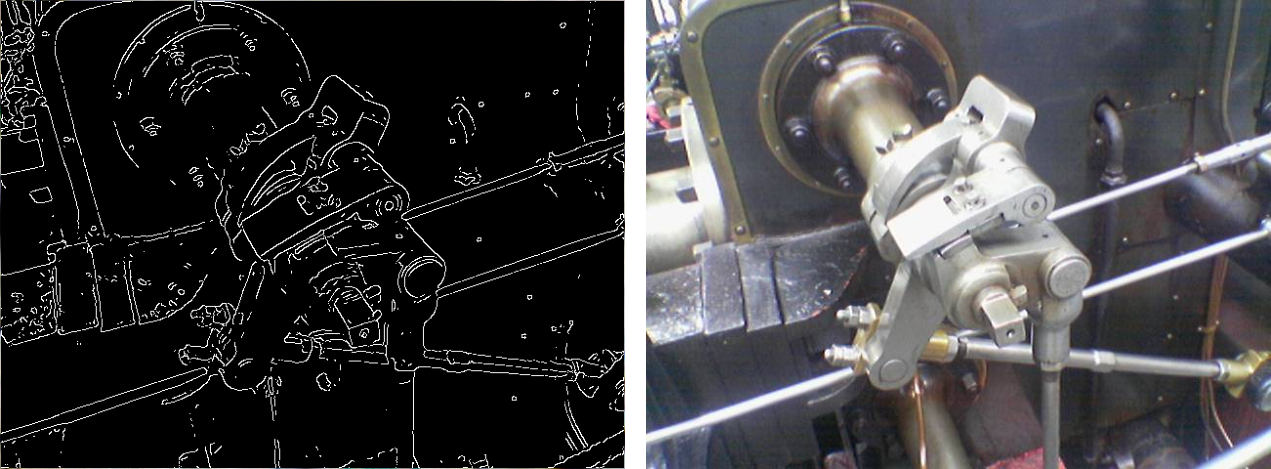
\includegraphics[width=\textwidth]{gfx/canny}
  \caption{\textbf{Lewy obraz:} Wynik zaaplikowanego algorytmu Canny na kolorowym obrazie z prawej strony. \textbf{Prawy obraz:} Oryginalny obraz.}
  \label{fig:algorytmy_korejestracji:canny}
\end{figure}

\end{itemize}

\subsubsection{Dopasowanie wyekstrahowanych cech}

Następnym krokiem po wyekstrahowaniu cech w dwóch obrazach jest ich dopasowanie na podstawie deskryptorów. Najprostszym rozwiązaniem może być porównanie każdej cechy z pierwszego obrazu do każdej cechy z drugiego obrazu, natomiast dla niektórych zastosowań jest to rozwiązanie zbyt wymagające obliczeniowo. Z tego względu zostały opracowane bardziej wydajne algorytmy. Przykładem jest wykorzystanie drzewa k-d przez Beis i Lowe \cite{Beis:1997}.

Kolejnym wyzwaniem w dopasowaniu cech jest wykrycie obserwacji odstających (ang. \textit{outliners}). Problem obrazuje rysunek \ref{fig:algorytmy_korejestracji:outliners}.

\begin{figure}[H]
  \centering
  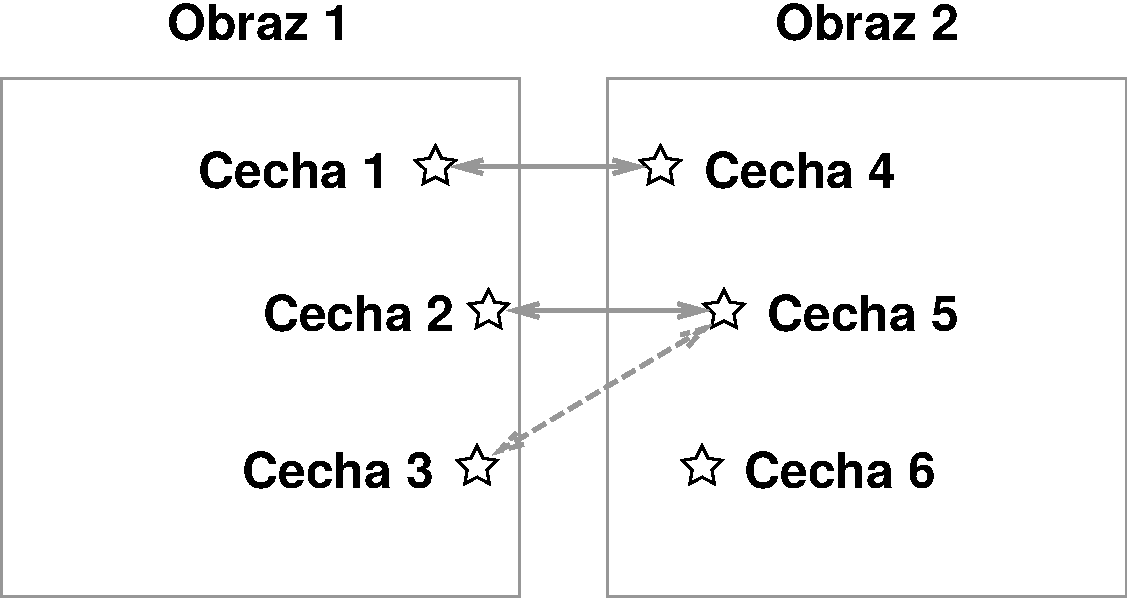
\includegraphics[width=6cm]{gfx/match}
  \caption{Dwa obrazy, w których wykryto po trzy cechy (na rysunku oznaczone jako gwiazdy). Algorytm szukający dopasowań wykrył dopasowania (na rysunku oznaczone jako strzałki) pomiędzy cechami: 1 i 4, 2 i 5, 3 i 5. Z wiedzy dziedzinowej wiemy, że obrazy nachodzą na siebie (tak jak angiograficzne obrazy OCT). Patrząc na dopasowania pomiędzy obrazami można zauważyć, że jedno z nich nie pasuje do reszty (strzałka narysowana przerywaną linią). Zakładając, że można tylko obracać i przesuwać obrazy niemożliwa jest estymacja macierzy transformacji biorąc pod uwagę wszystkie dopasowania. Niepoprawne dopasowanie trzeba odrzucić by otrzymać poprawną macierz transformacji.}
  \label{fig:algorytmy_korejestracji:outliners}
\end{figure}

Problem z rysunku \ref{fig:algorytmy_korejestracji:outliners} można rozwiązać poprzez odpowiednie filtrowanie dopasowań. Jedną z takich metod jest RANSAC (ang. \textit{random sample consensus, RANSAC}), który jest algorytmem iteracyjnym i jego zadaniem jest eliminacja obserwacji odstających. RANSAC jest wykorzystywany w niniejszej pracy i jest dokładniej opisy w sekcji \ref{sec:proponowane_algorytmy:ransac}. Do rozwiązania tego problemu można również wykorzystać relacje geometryczne pomiędzy obrazami. Relacje geometryczne definiuje się na podstawie wiedzy dziedzinowej (np. obraz nie może się przesunąć dalej niż 10 pikseli -- wszystkie dopasowania cech znajdujące się dalej niż 10 pikseli są niepoprawne). Filtracja na podstawie wiedzy dziedzinowej jest wykorzystywana w niniejszej pracy i jest opisana dokładniej w sekcji \ref{sec:proponowane_algorytmy:filtrowanie}.

\subsubsection{Estymacja macierzy transformacji na podstawie dopasowań}

Następnym krokiem po wyznaczeniu dopasowań pomiędzy dwoma obrazami jest estymacja macierzy transformacji jednego obrazu względem drugiego. Estymacja macierzy transformacji wykonuje się na podstawie ustalonego modelu deformacji (sekcja \ref{sec:algorytmy_korejestracji:model_deformacji}). Biorąc pod uwagę jako model transformacji ciało sztywne (dozwolona rotacja i translacja) równanie pozwalające obliczyć parametry rotacji i translacji można zapisać jako:
\begin{equation}
T=SR+t
\end{equation}
gdzie $T$ to zbiór cech w obrazie docelowym, $S$ to zbiór cech w obrazie źródłowym, $R$ to macierz rotacji, a $t$ to wektor translacji. Wyznaczenie $R$ i $t$ z tego równania byłoby proste, jeżeli wszystkie cechy z obrazu źródłowego dałoby się idealnie przekształcić na cechy obrazu docelowego. Istnieje bardzo mała szansa, że macierz transformacji obliczona na podstawie jednego dopasowania zaaplikowana do cechy z innego dopasowania zwróciłaby miejsce odpowiadającej cechy z drugiego obrazu (będzie blisko niej, ale nie idealnie w tym samym miejscu). Różnica wynika z tego, że obrazy posiadają szum oraz algorytmy zwracające cechy nie są tak dokładne. Jednym z prostszych rozwiązań tego problemu jest wykorzystanie metody minimalizacji błędu średniokwadratowego polegającej na znalezieniu takiej macierzy transformacji dla której błąd średniokwadratowy pomiędzy cechą w obrazie docelowym, a cechą z obrazu źródłowego po transformacji jest najmniejszy. Mając dane współrzędne cechy w obrazie docelowym $T_{i}$ oraz współrzędne odpowiadającej cechy w obrazie źródłowym $S_{i}$ oraz macierz transformacji $M$ błąd średniokwadratowy można zapisać jako:
\begin{equation}
E_{LS}=\sum_{i}d(T_{i}, MS_{i})^2
\label{eq:estimate}
\end{equation}
gdzie $E_{LS}$ to minimalny błąd średniokwadratowy, a funkcja $d(...)$ to odległość euklidesowa pomiędzy dwoma punktami.

Równanie \ref{eq:estimate} można rozwiązać algorytmami optymalizacji. W niniejszej pracy do wyznaczenia parametrów rotacji i translacji na podstawie dopasowań została wykorzystana funkcja OpenCV, której użycie jest opisane w sekcji \ref{sec:proponowane_algorytmy:estymacja}.

\section{Łączenie kafelków}
\label{sec:algorytmy_korejestracji:laczenie_kafelkow}

Po wyznaczeniu macierzy translacji pomiędzy dwoma kafelkami następnym krokiem jest ich złączenie w obszarze, w którym na siebie nachodzą. Problem by nie istniał jeżeli dopasowanie byłoby idealne oraz ekspozycja dwóch kafelków byłaby identyczna. Niestety w rzeczywistym świecie po złączeniu widoczne są krawędzie kafelków oraz inne artefakty wynikające z błędu rejestracji, czy niedokładności aparatu. Stworzenie ładnej oraz jednorodnej mozaiki wymaga określenia, które piksele z dwóch kafelków należy wykorzystać w procesie łączenia oraz jakie przypisać im wagi. Najprostszą metodą jest wzięcie średniej ważonej każdego piksela z dwóch łączonych kafelków:
\begin{equation}
f(x)=\frac{\sum_{i}\omega_{i}(x)f_{i}(x)}{\sum_{i}\omega_{i}(x)}
\label{eq:blending}
\end{equation}
gdzie $i$ to liczba nakładających się kafelków, $f(x)$ to wartość piksela $x$ w finalnej mozaice, $f_{i}(x)$ to wartość piksela $x$ w kolejnych nakładających się kafelkach, a $w(x)$ to waga piksela $x$. Następnym krokiem w tej metodzie jest ustalenie wartości wag. Jednym z pomysłów jest wykorzystanie zwykłej średniej ($w(x)=1$ dla każdego piksela $x$). Nie jest to jednak najlepszy sposób, ponieważ krawędzie kafelków po zastosowaniu średniej są dalej widoczne. Lepszym podejściem jest uzależnienie wartości wag od odległości piksela od środka kafelka do którego należy (piksel znajdujący się przy krawędzi swojego kafelka będzie miał mniejszą wagę niż piksel znajdujący się blisko środka swojego kafelka). Metoda wykorzystana jest w niniejszej pracy i dokładniej jest opisana w sekcji \ref{sec:proponowane_algorytmy:laczenie_kafelkow}. Istnieją również bardziej zaawansowane metody takie jak algorytm \textit{multi-band blending} zaproponowany przez Burt i Adelson \cite{Burt:1983:MSA:245.247} dający jeszcze lepsze rezultaty \cite{Brown:2007:API:1265138.1265141}.

















